\documentclass[12pt, a4paper]{report}
\usepackage[utf8]{inputenc}
\usepackage[russian]{babel}
\usepackage{listings}
\usepackage{graphicx}
\usepackage{amsmath,amsfonts,amssymb,amsthm,mathtools} 
\usepackage{float}
\usepackage{pdfpages}

% Для листинга кода:
\lstset{ %
language=python,                   % выбор языка для подсветки
basicstyle=\small\sffamily, 	  % размер и начертание шрифта для подсветки кода
numbers=left,               		  % где поставить нумерацию строк (слева\справа)
numberstyle=\tiny,           		% размер шрифта для номеров строк
stepnumber=1,                        % размер шага между двумя номерами строк
numbersep=7pt,                      % как далеко отстоят номера строк от подсвечиваемого кода
showspaces=false,                  % показывать или нет пробелы специальными отступами
showstringspaces=false,         % показывать или нет пробелы в строках
showtabs=false,                      % показывать или нет табуляцию в строках
frame=single,                           % рисовать рамку вокруг кода
tabsize=4,                 				  % размер табуляции по умолчанию равен 2 пробелам
captionpos=b,                           % позиция заголовка вверху [t] или внизу [b] 
breaklines=true,                        % автоматически переносить строки (да\нет)
breakatwhitespace=false,          % переносить строки только если есть пробел
escapeinside={\#*}{*)}               % если нужно добавить комментарии в коде
}

% Для измененных титулов глав:
\usepackage{titlesec, blindtext, color} % подключаем нужные пакеты
\definecolor{gray75}{gray}{0.75} % определяем цвет
\newcommand{\hsp}{\hspace{20pt}} % длина линии в 20pt
% titleformat определяет стиль
\titleformat{\chapter}[hang]{\Huge\bfseries}{\thechapter\hsp\textcolor{gray75}{|}\hsp}{0pt}{\Huge\bfseries}


% plot
\usepackage{pgfplots}
\usepackage{filecontents}
\usetikzlibrary{datavisualization}
\usetikzlibrary{datavisualization.formats.functions}
\begin{filecontents}{lr.dat}
1 3222
2 12329
3 51963
4 285784
5 1503606
6 8650819
7 56342756
\end{filecontents}

\begin{filecontents}{lm.dat}
1 5316
2 9482
3 13505
4 22975
5 33575
6 51708
7 83139
\end{filecontents}

\begin{filecontents}{ldr.dat}
1 3477
2 13058
3 55535
4 305489
5 1601602
6 9243470
7 59932134
\end{filecontents}

\begin{filecontents}{ldm.dat}
1 5292
2 9867
3 14453
4 25249
5 37265
6 58086
7 93704
\end{filecontents}


\begin{filecontents}{lrmem.dat}
1 504
2 2410
3 11950
4 61210
5 321372
6 1717362
7 9295242
\end{filecontents}

\begin{filecontents}{lmmem.dat}
1 244
2 246
3 248
4 282
5 284
6 286
7 288
\end{filecontents}

\begin{filecontents}{ldrmem.dat}
1 532
2 2578
3 12818
4 65690
5 344920
6 1843194
7 9976174
\end{filecontents}

\begin{filecontents}{ldmmem.dat}
1 244
2 246
3 248
4 282
5 284
6 286
7 288
\end{filecontents}


\begin{document}

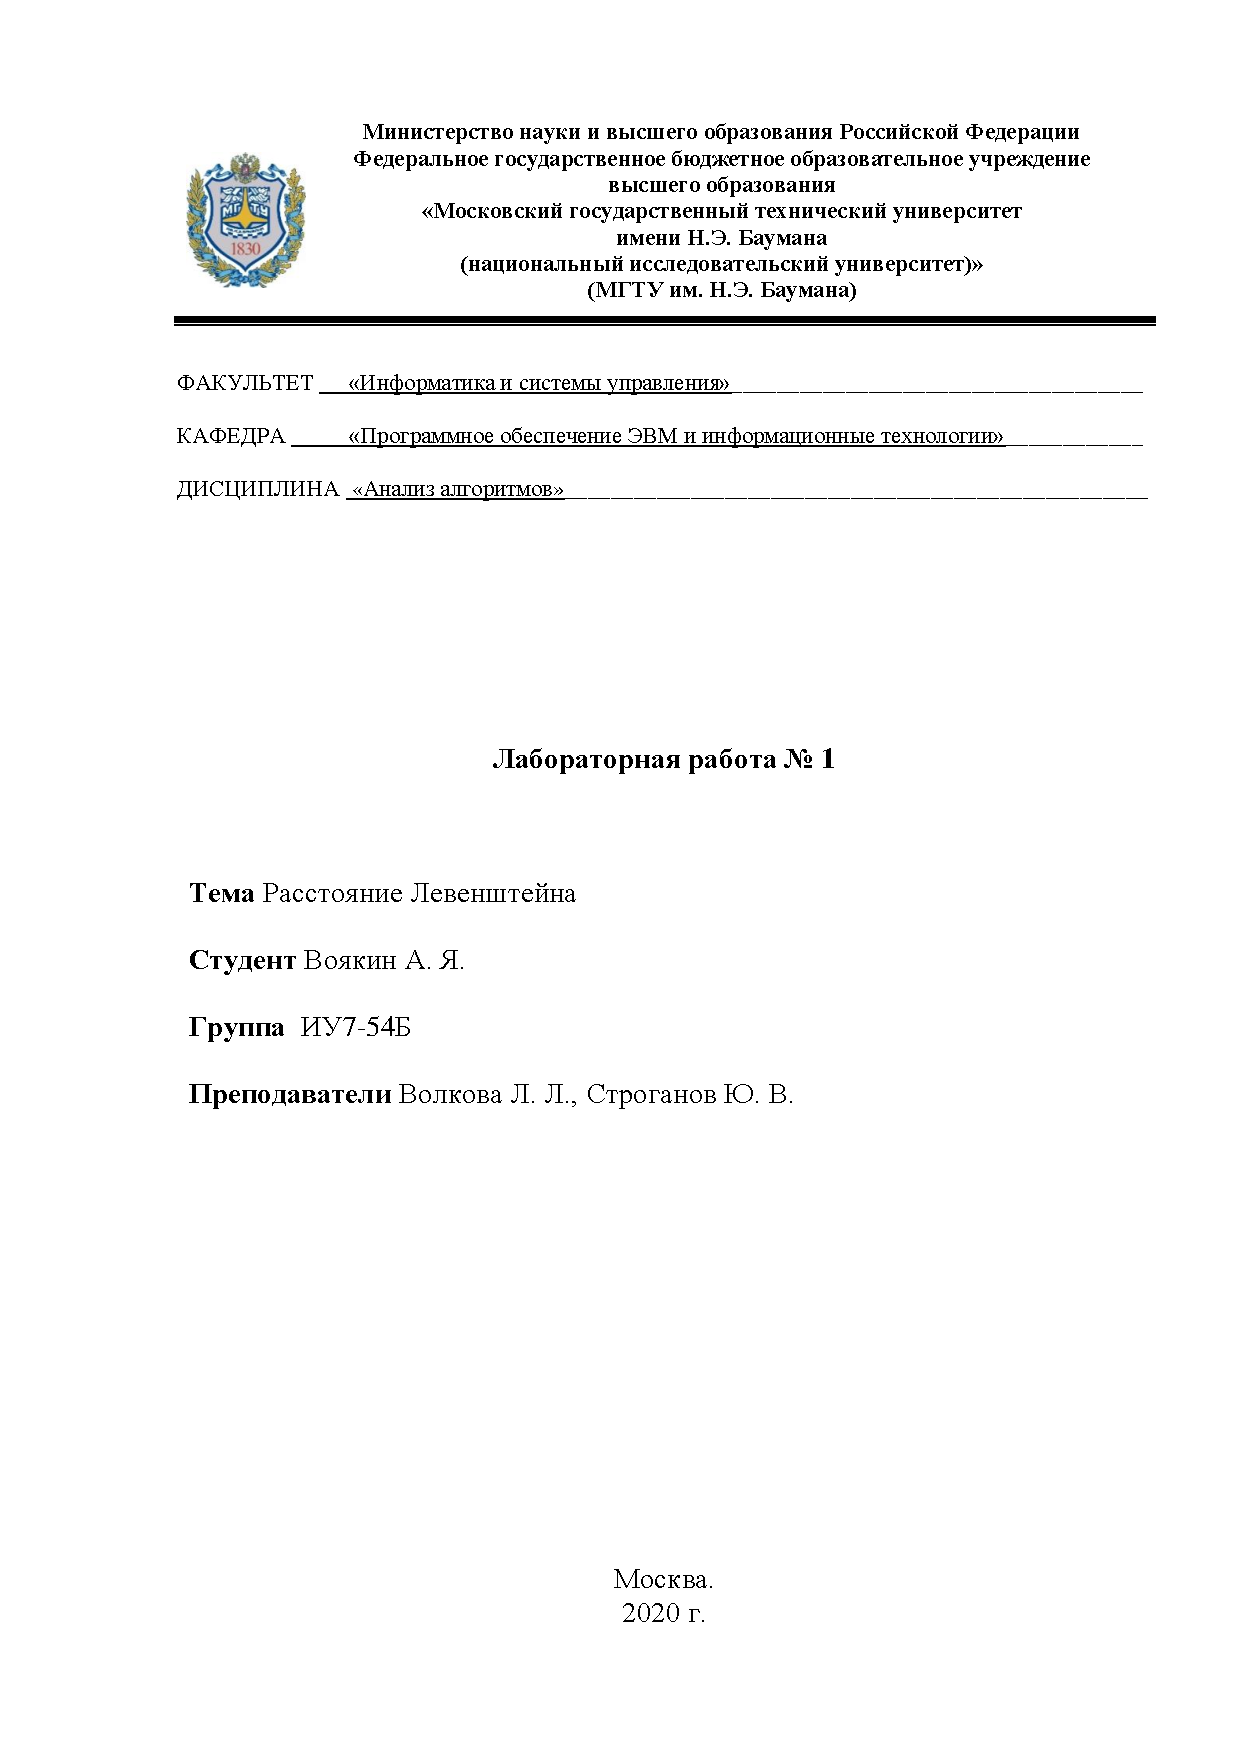
\includepdf{Title.pdf}

\tableofcontents

\newpage
\chapter*{Введение}
\addcontentsline{toc}{chapter}{Введение}
\textbf{Расстояние Левенштейна} - согласно [4] - минимальное количество операций вставки одного символа, удаления одного символа и замены одного символа на другой, необходимых для превращения одной строки в другую.

Расстояние Левенштейна применяется в теории информации и компьютерной лингвистике для:

\begin{itemize}
	\item исправления ошибок в слове;
	\item сравнения текстовых файлов (утилита diff);
	\item в биоинформатике для сравнения генов, хромосом и белков.
\end{itemize}

Целью данной лабораторной работы является изучение метода динамического программирования на примере алгоритмов
Левенштейна и Дамерау-Левенштейна. 

Задачами лабораторной работы являются:
\begin{itemize}
  	\item изучение алгоритмов Левенштейна и Дамерау-Левенштейна нахождения расстояния между строками;
	\item реализация рекурсивной и динамической вариации указанных алгоритмов; 
	\item тестирование реализованных алгоритмов; 
	\item проведение сравнительного анализа алгоритмов по затрачиваемым ресурсам (времени и памяти).
\end{itemize}


\chapter{Аналитическая часть}
		\section{Описание алгоритмов}
Задача по нахождению расстояния Левенштейна заключается в поиске минимального количества операций вставки/удаления/замены для превращения одной строки в другую.

При нахождении расстояния Дамерау — Левенштейна добавляется операция транспозиции (перестановки соседних символов). Полное определение рассмотрено в [1].  
 
\textbf{Действия обозначаются так:} 
\begin{itemize}
  	\item D (англ. delete) — удалить;
	\item I (англ. insert) — вставить;
	\item R (replace) — заменить;
	\item M(match) - совпадение.
\end{itemize}

Пусть $S_{1}$ и $S_{2}$ — две строки (длиной M и N соответственно) над некоторым алфавитом, тогда расстояние Левенштейна можно подсчитать по рекуррентной формуле (1.1), см [3]:


\begin{equation}
D(i,j) = \left\{ \begin{array}{ll}
 0, & \textrm{$i = 0, j = 0$}\\
 i, & \textrm{$j = 0, i > 0$}\\
 j, & \textrm{$i = 0, j > 0$}\\
min(\\
D(i,j-1)+1,\\
D(i-1, j) +1, &\textrm{$j>0, i>0$}\\
D(i-1, j-1) + m(S_{1}[i], S_{2}[j])\\
),
\end{array} \right.
\end{equation}

где $m(a,b)$ равна нулю, если $a=b$ и единице в противном случае; $min\{\,a,b,c\}$ возвращает наименьший из аргументов.

Расстояние Дамерау-Левенштейна вычисляется по рекуррентной формуле (1.2), см [2]:
		\begin{equation}
		     D(i, j) =  \left\{
			\begin{aligned}
				&0, && i = 0, j = 0\\
		    	&i, && i > 0, j = 0\\
		    	&j, && i = 0, j > 0\\		    	
		    	&min \left\{
				\begin{aligned}
					&D(i, j - 1) + 1,\\
		            &D(i - 1, j) + 1,\\
		            &D(i - 1, j - 1) + m(S_{1}[i], S_{2}[i]), \\
		            &D(i - 2, j - 2) + m(S_{1}[i], S_{2}[i]),\\
		        \end{aligned} \right.
		        && 
				\begin{aligned}
					&, \text{ если } i, j > 0 \\
		            & \text{ и } S_{1}[i] = S_{2}[j - 1] \\
		            & \text{ и } S_{1}[i - 1] =  S_{2}[j] \\
		        \end{aligned} \\ 
		        &min \left\{
		        \begin{aligned}
		            &D(i, j - 1) + 1,\\
		            &D(i - 1, j) + 1, \\
		            &D(i - 1, j - 1) + m(S_{1}[i], S_{2}[i]),\\
		        \end{aligned} \right.  &&, \text{иначе}
			\end{aligned} \right.
		\end{equation}

Недостатком использования рекуррентных формул для измерения редакционного расстояния являются повторные вчисления. 
Решением данного недостатка является использование матричного алгоритма. Для хранения используется матрица размером (len(S1) + 1 x len(S2) + 1).
\section{Вывод}
В данном разделе были рассмотрены алгоритмы нахождения расстояния Левенштейна и Дамерау-Левенштейна, который является модификаций первого, учитывающего возможность перестановки соседних символов. 
 



\chapter{Конструкторская часть}
\section{Техническое задание}
\textbf{Ввод:}
\begin{itemize}
  	\item на вход подаются две строки;
  	\item строки могут быть пустыми, содержать пробелы, а также любые печатные символы UTF-8;
	\item uppercase и lowercase буквы считаются разными.
\end{itemize}
\textbf{Вывод:}
\begin{itemize}
  	\item программа выводит посчитанные каждым из алгоритмов расстояния;
  	\item для динамических реализаций алгоритмов выводятся заполненные матрицы;
  	\item в режиме замера ресурсов программа выводит средние время и память, затраченные каждым алгоритмом. 
\end{itemize}
\section{Разработка алгоритмов}
В данной части будут рассмотрены схемы алгоритмов Схемы рекурсивного алгоритма нахождения расстояния Левенштейна, матричного алгоритма нахождения расстояния Левенштейна, рекурсивного алгоритма нахождения расстояния Дамерау-Левенштейна и матричного алгоритма нахождения расстояния Дамерау-Левенштейна показаны на рисунках 2.1, 2.2, 2.3 и 2.4, соответственно.

\begin{figure}[h]
\centering
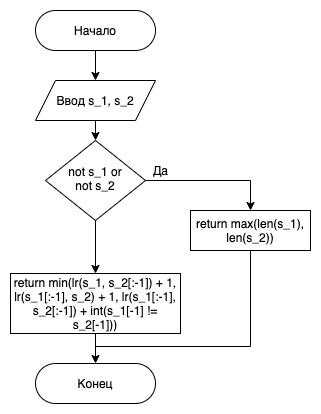
\includegraphics[width=0.8\linewidth]{lr.jpg}
\caption{Схема рекурсивного алгоритма нахождения расстояния Левенштейна}
\label{fig:mpr}
\end{figure}

\begin{figure}[h]
\centering
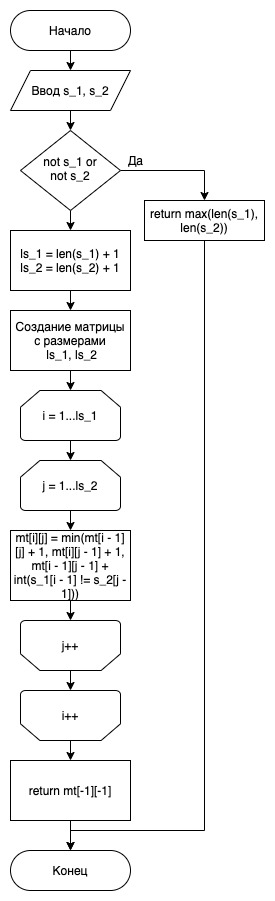
\includegraphics[width=0.44\linewidth]{lm.jpg}
\caption{Схема матричного алгоритма нахождения расстояния Левенштейна}
\label{fig:mpr}
\end{figure}

\begin{figure}[h]
\centering
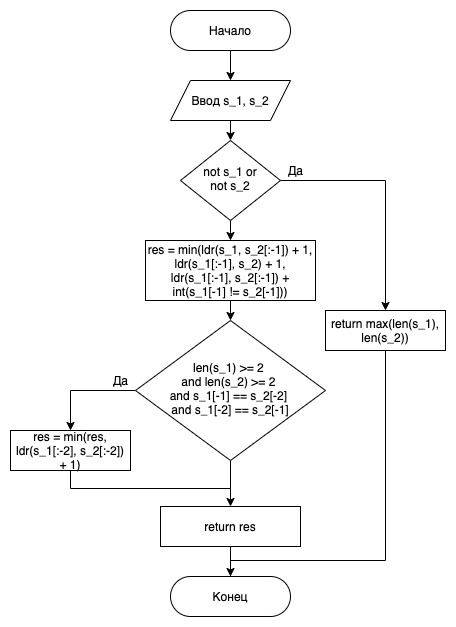
\includegraphics[width=0.9\linewidth]{ldr.jpg}
\caption{Схема рекурсивного алгоритма нахождения расстояния Дамерау-Левенштейна}
\label{fig:mpr}
\end{figure}

\begin{figure}[h]
\centering
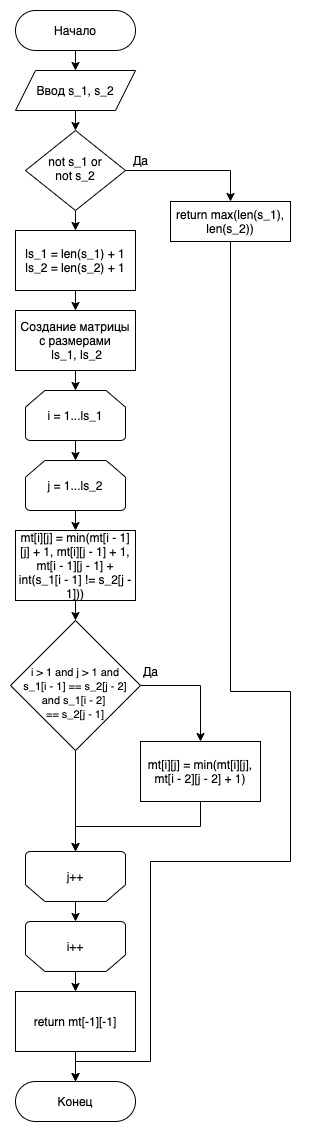
\includegraphics[width=0.4\linewidth]{ldm.jpg}
\caption{Схема матричного алгоритма нахождения расстояния Дамерау-Левенштейна}
\label{fig:mpr}
\end{figure}


\chapter{Технологическая часть}
\section{Выбор ЯП}
Для реализации программы был выбран Python из-за наличия опыта разработки на данном языке программирования. Среда разработки - PyCharm.


\section{Реализация алгоритма}

\begin{lstlisting}[label=some-code,caption=Функция нахождения расстояния Левенштейна рекурсивно]
def lr(s_1, s_2):
	if not s_1 or not s_2:
		return max(len(s_1), len(s_2))
	return min(lr(s_1, s_2[:-1]) + 1, 
					 lr(s_1[:-1], s_2) + 1, 
					 lr(s_1[:-1], s_2[:-1]) + int(s_1[-1] != s_2[-1]))
\end{lstlisting}

\begin{lstlisting}[label=some-code,caption=Функция нахождения расстояния Левенштейна матрично]
def lm(s_1, s_2, return_matrix=False):
	if not s_1 or not s_2:
		return max(len(s_1), len(s_2))
	ls_1 = len(s_1) + 1
	ls_2 = len(s_2) + 1
	mt = [[i + j for j in range(ls_2)] for i in range(ls_1)]
	for i in range(1, ls_1):
		for j in range(1, ls_2):
			mt[i][j] = min(mt[i - 1][j] + 1, mt[i][j - 1] + 1, mt[i - 1][j - 1] + int(s_1[i - 1] != s_2[j - 1]))
	if return_matrix:
		return mt
	return mt[-1][-1]
\end{lstlisting}


\begin{lstlisting}[label=some-code,caption=Функция нахождения расстояния Дамерау-Левенштейна рекурсивно]
def ldr(s_1, s_2):
	if not s_1 or not s_2:
		return max(len(s_1), len(s_2))
	res = min(ldr(s_1, s_2[:-1]) + 1, ldr(s_1[:-1], s_2) + 1, ldr(s_1[:-1], s_2[:-1]) + int(s_1[-1] != s_2[-1]))
	if len(s_1) >= 2 and len(s_2) >= 2 and s_1[-1] == s_2[-2] and s_1[-2] == s_2[-1]:
		res = min(res, ldr(s_1[:-2], s_2[:-2]) + 1)
	return res
\end{lstlisting}

\begin{lstlisting}[label=some-code,caption=Функция нахождения расстояния Дамерау-Левенштейна матрично]
def ldm(s_1, s_2, return_matrix=False):
	if not s_1 or not s_2:
		return max(len(s_1), len(s_2))
	ls_1 = len(s_1) + 1
	ls_2 = len(s_2) + 1
	mt = [[i + j for j in range(ls_2)] for i in range(ls_1)]
	for i in range(1, ls_1):
		for j in range(1, ls_2):
			mt[i][j] = min(mt[i - 1][j] + 1, mt[i][j - 1] + 1, mt[i - 1][j - 1] + int(s_1[i - 1] != s_2[j - 1]))
			if i > 1 and j > 1 and s_1[i - 1] == s_2[j - 2] and s_1[i - 2] == s_2[j - 1]:
				mt[i][j] = min(mt[i][j], mt[i - 2][j - 2] + 1)
	if return_matrix:
		return mt
	return mt[-1][-1]
\end{lstlisting}

\begin{lstlisting}[label=some-code,caption=Функция вывода матрицы на экран]
def mt_print(mt):
	if type(mt) == list:
		for row in mt:
			print(' '.join(map(str, row)))
	else:
		print("Matrix not used.")
\end{lstlisting}

\begin{lstlisting}[label=some-code,caption=Измерение процессорного времени выполнения алгоритмов]
print("| len |   LevRec   |   LevMat   |   LevDamRec   |   LevDamMat   |")
for i in range(1, 8):
	s_1 = ''.join(sample(ascii_letters, i))
	s_2 = ''.join(sample(ascii_letters, i))
	lr_time_arr = []
	lm_time_arr = []
	ldr_time_arr = []
	ldm_time_arr = []
	for _ in range(1000):
		lr_time_arr.append(cpu_time(alg.lr, s_1, s_2))
		lm_time_arr.append(cpu_time(alg.lm, s_1, s_2))
		ldr_time_arr.append(cpu_time(alg.ldr, s_1, s_2))
		ldm_time_arr.append(cpu_time(alg.ldm, s_1, s_2))
	print("%5d" % i, "%12d" % int(sum(lr_time_arr) / len(lr_time_arr)),
			"%12d" % int(sum(lm_time_arr) / len(lm_time_arr)),
			"%15d" % int(sum(ldr_time_arr) / len(ldr_time_arr)),
			"%15d" % int(sum(ldm_time_arr) / len(ldm_time_arr)))
\end{lstlisting}

\begin{lstlisting}[label=some-code,caption=Функция замера процессорного времени]
def cpu_time(func, s_1, s_2):
	start = process_time_ns()
	func(s_1, s_2)
	end = process_time_ns()
	return end - start
\end{lstlisting}

\chapter{Исследовательская часть}

\section{Сравнительный анализ на основе замеров времени работы алгоритмов}

Был проведен замер времени работы каждого из алгоритмов. 
Для замера времени генерировались две различные строки необходимой длины.
Результаты представленные в таблице 4.1 получены усреднением значений каждого алгорима,  выполненного 1000 раз при одинаковых входных данных.

\begin{table} [ht]
	\caption{Время работы алгоритмов в нано секундах.}
\begin{center}
\begin{tabular}{|c c c c c|} 
 	\hline
	len & LevRec & LevMat & LevDamRec & LevDamMat \\ [0.8ex] 
 	\hline
 	1 & 3222 & 5316 & 3477 & 5292\\
 	\hline
 	2 & 12329 & 9482 & 13058 & 9867\\
 	\hline
	3 & 51963&13505&55535&14453\\
	\hline
	4 & 285784&22975&305489&25249\\
	\hline
	5 & 1503606&33575&1601602&37265\\
	\hline
	6 & 8650819&51708&9243470&58086\\
	\hline
	7 & 56342756&83139&59932134&93704\\
	\hline
	\end{tabular}
\end{center}
\end{table}

Полученная зависимость времени работы алгоритмов от длины строк показана на рисунках 4.1, 4.2.


\begin{figure} [H]
\begin{center}
\begin{tikzpicture}
\begin{axis}[
    	axis lines = left,
    	xlabel={Длина строк},
    	ylabel={Время в нано секундах},
    	xmin=1, xmax=7,
    	ymin=1, ymax=55000000,
	legend pos=north west,
	ymajorgrids=true
]
\addplot[color=red] table[x index=0, y index=1] {lr.dat}; 
\addplot[color=orange] table[x index=0, y index=1] {ldr.dat};

\addlegendentry{LevRec}
\addlegendentry{LevDamRec}
\end{axis}
\end{tikzpicture}
\caption{Зависимость времени работы рекурсивных реализаций алгоритмов от длины строк}
\end{center}
\end{figure}

\begin{figure} [H]
	\begin{center}
		\begin{tikzpicture}
			\begin{axis}[
				axis lines = left,
				xlabel={Длина строк},
				ylabel={Время в нано секундах},
				xmin=1, xmax=7,
				ymin=1, ymax=100000,
				legend pos=north west,
				ymajorgrids=true
				]
				\addplot[color=blue, mark=square] table[x index=0, y index=1] {lm.dat};
				\addplot[color=green, mark=square] table[x index=0, y index=1] {ldm.dat};
				
				\addlegendentry{LevMat}
				\addlegendentry{LevDamMat}
			\end{axis}
		\end{tikzpicture}
		\caption{Зависимость времени работы матричных реализаций алгоритмов от длины строк}
	\end{center}
\end{figure}

\par
На основе проведённых измерений можно сделать вывод, что рекурсивные алгоритмы эффективней для коротких строк. Однако при увелечении длины, динамические алгоритмы выступают более эффективными, что обусловлено большим количеством повторных рассчетов в рекурсивных реализациях, в то время как в динамических реализациях ячейка матрицы расчитывается единожды. Также установлено, что алгоритм Дамерау Левенштейна в среднем работает несколько дольше алгоритма Левенштейна, что объясняется наличием дополнительных проверок, однако алгоритмы сравнимы по временной эффективности.



\section{Сравнительный анализ алгоритмов на основе замеров затрачиваемой памяти}
Был проведен замер памяти, затрачиваемой алгоритмами. Результат замера показан в таблице 4.2.


\begin{table} [H]
	\caption{Затрачиваемая алгоритмами память в байтах}
	\begin{center}
	\begin{tabular}{|c c c c c|} 
		\hline
		len & LevRec & LevMat & LevDamRec & LevDamMat \\ [0.8ex] 
		\hline
		1 & 504&244  &           532 &            244\\
		\hline
		2 & 2410     &     246      &      2578     &        246\\
		\hline
		3 & 11950      &    248       &    12818     &        248\\
		\hline
		4 & 61210        &  282         &  65690      &       282\\
		\hline
		5 & 321372       &   284         & 344920     &        284\\
		\hline
		6 & 1717362        &  286    &     1843194      &       286\\
		\hline
		7 & 9295242         & 288     &    9976174       &      288\\
		\hline
	\end{tabular}
	\end{center}
	
\end{table}



Полученная зависимость памяти, затрачиваемой алгоритмами, от длины строк показана на рисунках 4.3, 4.4.

\begin{figure} [H]
\begin{center}
	\begin{tikzpicture}
		\begin{axis}[
			axis lines = left,
			xlabel={Длина строк},
			ylabel={Кол-во памяти в байтах},
			xmin=1, xmax=7,
			ymin=1, ymax=10000000,
			legend pos=north west,
			ymajorgrids=true
			]
			\addplot[color=red] table[x index=0, y index=1] {lrmem.dat}; 
			\addplot[color=orange] table[x index=0, y index=1] {ldrmem.dat};
			
			\addlegendentry{LevRec}
			\addlegendentry{LecDamRec}
		\end{axis}
	\end{tikzpicture}
\end{center}
	\caption{Зависимость затрачиваемой памяти рекурсивными реализациями алгоритмов от длины строк}
\end{figure}

\begin{figure} [H]
	\begin{center}
		\begin{tikzpicture}
			\begin{axis}[
				axis lines = left,
				xlabel={Длина строк},
				ylabel={Кол-во памяти в байтах},
				xmin=1, xmax=7,
				ymin=200, ymax=320,
				legend pos=north west,
				ymajorgrids=true
				]
				\addplot[color=blue, mark=square] table[x index=0, y index=1] {lmmem.dat};
				\addplot[color=green, mark=square] table[x index=0, y index=1] {ldmmem.dat};
				
				\addlegendentry{LevMat}
				\addlegendentry{LevDamMat}
			\end{axis}
		\end{tikzpicture}
	\end{center}
	\caption{Зависимость затрачиваемой памяти матричными реализациями алгоритмов от длины строк}
\end{figure}

\par
На основе проведённых измерений можно сделать вывод, что рекурсивные алгоритмы сравнимы по количеству затрачиваемой памяти с динамическими при малых длинах входных строк. Однако при росте длины строк количество памяти, затрачиваемой рекурсивными алгоритмами резко возрастает из-за локальных переменных, создаваемых при каждом вызове алгоритма, в то время как память динамических алгоритмов изменяется слабо - только из-за увеличения хранимой матрицы.




\section{Тестовые данные}

\par
Проведем тестирование программы. В столбцах "Ожидаемый результат" и "Полученный результат" 4 числа соответсвуют рекурсивному алгоритму нахождения расстояния Левенштейна, матричному алгоритму нахождения расстояния Левенштейна, рекурсивному алгоритму расстояния Дамерау-Левенштейна, матричному алгоритму нахождения расстояние Дамерау-Левенштейна.

\begin{table} [H]
\begin{center}
	\caption{Таблица тестовых данных}
	\begin{tabular}{|c c c c c|} 
 	\hline
	№ &  Строка № 1 & Строка № 1 & Ожидаемый рез. & Полученный рез. \\ [0.8ex] 
 	\hline
 	1 &  &  & 0 0 0 0 & 0 0 0 0\\
 	\hline
 	2 & help & me & 3 3 3 3 & 3 3 3 3\\
 	\hline
	3 & Im & tired & 5 5 5 5  & 5 5 5 5\\
	\hline
	4 & pen & pne & 2 2 1 1 & 2 2 1 1\\
	\hline
	5 &  & empty & 5 5 5 5 & 5 5 5 5\\
	\hline
	6 & 123 &  & 3 3 3 3 & 3 3 3 3\\
	\hline
	7 & Я & русский & 7 7 7 7  & 7 7 7 7\\
	\hline
	8 & еен & ене & 2 2 1 1 & 2 2 1 1\\
	\hline
	\end{tabular}
\end{center}
\end{table}



\chapter*{Заключение}
\addcontentsline{toc}{chapter}{Заключение}
Были изучены методы динамического и рекурсивного программирования на примере алгоритмов Левенштейна и Дамерау-Левенштейна. Получены практические навыки реализации указанных алгоритмов в матричной и динамической реализации.

Экспериментально было подтверждено различие во временной эффективности рекурсивной и нерекурсивной реализаций выбранного алгоритма определения расстояния между строками при помощи разработаного программного обеспечения на материале замеров процессорного времени выполнения реализации на варьирующихся длинах строк. 

В результате исследований можно прийти к вводу, что матричная реализация данных алгоритмов заметно выигрывает по времени при росте длины строк, следовательно более применима в реальных проектах.


\chapter*{Список использованных источников}
\begin{enumerate}
	\item Задача о расстоянии Дамерау-Левенштейна [Электронный ресурс]. – Режим доступа: https://neerc.ifmo.ru/wiki/index.php?title=Задача-о-расстоянии-Дамерау-Левенштейна. – Дата доступа: 27.10.2020.
	\item Вычисление редакционного расстояния [Электронный ресурс]. – Режим доступа: https://habr.com/ru/post/117063/. – Дата доступа: 27.10.2020.
	\item Вычисление расстояния Левенштейна [Электронный ресурс]. – Режим доступа: https://foxford.ru/wiki/informatika/vychislenie-rasstoyaniya-levenshteyna. – Дата доступа: 27.10.2020.
	\item Расстояние Левенштейна [Электронный ресурс]. – Режим доступа: https://vc.ru/newtechaudit/129654-rasstoyanie-levenshteyna-dlya-poiska-opechatok-v-dannyh-klienta. – Дата доступа: 27.10.2020.
\end{enumerate}
\end{document}